\section{Umsetzung des Projektziels}\label{umsetzungProjekt}
Dieses Kapitel behandelt nun die konkrete Umsetzung des eigentlichen Projektziels "Man-In-The-Middle". Der Ansatz besteht darin die Gesprächsdaten auf der Strecke zwischen BTS, BSC und der Telefonvermittlungsanlage abzugreifen und zu speichern. Da alle Systeme softwareseitig auf einem PC ausgeführt werden und diese über Sockets miteinander kommunizieren, können die Daten überall abgegriffen werden.\\

Für die Installation und Einrichtung der benötigten Tools wurde ein Bash-Skript erstellt, welches die meisten Schritte automatisch durchführt. Die manuell noch auszuführenden Schritte werden in der Komandozeile ebenfalls ausgegeben (Skript siehe Anhang \ref{configureScript}).


\subsection{Abspeichern der Daten}\label{abspeichern}
Mit Wireshark oder den beiden Komandozeilenanwendungen tshark und tcpdump können Daten von einem Interface analysiert werden und auch in eine pcap-Datei abgespeichert werden. Hierbei können bereits bei der Aufnahme Filter gesetzt werden, sodass nur die relevanten Daten gespeichert werden.\\

Pcapsipdump ist ein open-source Tool, welches auf \textit{libpcap} basiert. Das Tool hört auf einem Interface den Netzwerkverkehr mit und speichert die SIP/RTP-Sessions als pcap-Datei ab. Diese Datei kann nun in tcpdump, Wireshark oder ähnlichem geöffnet, eingelesen und weiterverarbeitet werden. Eine hilfreiche Eigenschaft von pcapsipdump ist, dass das Tool pro Session selbstständig eine neue Datei anlegt. Das Tool läuft als Hintergrundprozess, sodass es nur einmal manuell gestartet werden muss. Alternativ kann pcapsipdump auch mit dem systemd-Init-Prozess automatisch gestartet werden, sofern man es nachträglich selbst konfiguriert. Da die Tools für das GSM-Netz, wie bereits erwähnt, alle auf demselben Rechner laufen, reicht es das Loopback-Interface abzuhören.\\

Vor der Installation des Programmes selbst muss Subversion und folgende Abhängigkeit installiert werden.
\begin{lstlisting}
sudo apt-get install -y subversion libpcap-dev
\end{lstlisting}

Das Programm selbst vom SVN-Server herunterladen und installieren.
\begin{lstlisting}
svn checkout https://svn.code.sf.net/p/pcapsipdump/code/trunk pcapsipdump-code
cd pcapsipdump-code
sudo make
sudo make install
\end{lstlisting}

Das Tool kann über das selbst erstellte startingPcapsipdump.sh-Skript oder alternativ auch manuell gestartet werden. Mit angegebenen Parametern lauscht es auf dem Loopback-Interface mit und speichert die Telefongespräche, sobald ein Anruf initiiert wird, in den angegeben Ordner. Des Weiteren werden die Daten immer Paket gepuffert geschrieben, sodass die pcap-Datei immer konsistent ist.
\begin{lstlisting}
sudo pcapsipdump -i lo -v 10 -d /home/all/wiresharkCalls/%Y%m%d-%H%M%S-%f-%t-%i.pcap -U
\end{lstlisting}

\subsection{Extrahieren und konvertieren der Daten}\label{extractData}
Zunächst wurden die von pcapsipdump extrahierten Daten mit Wireshark manuell analysiert. Darin sind nun nur noch die SIP- und RTP-Packet enthalten, wie in Abbildung \ref{fig:wSipRTP} zu sehen. Wireshark erkennt den VOIP-Anruf und kombiniert die RTP-Packages korrekt. Allerdings konnte der Stream nicht direkt im Programm abgespielt werden. Der Grund hierfür ist, dass Wireshark gsm nicht dekodieren kann.
Jedoch gibt es einen Weg, wie die beiden Streams als .raw-Daten exportiert werden können. Hierfür wird ein beliebiges RTP-Packet ausgewählt. Über die Menüoption \textit{Telefonie->RTP->Stream Analyse} kann der Stream analysiert werden. Nun kann der Hinweg und Rückweg als seperate Datei gespeichert werden. Man muss jedoch als Datei-Typ .raw auswählen.\\

\begin{figure}[h] %t=top b=bottom h=here p =eigene page
\centering
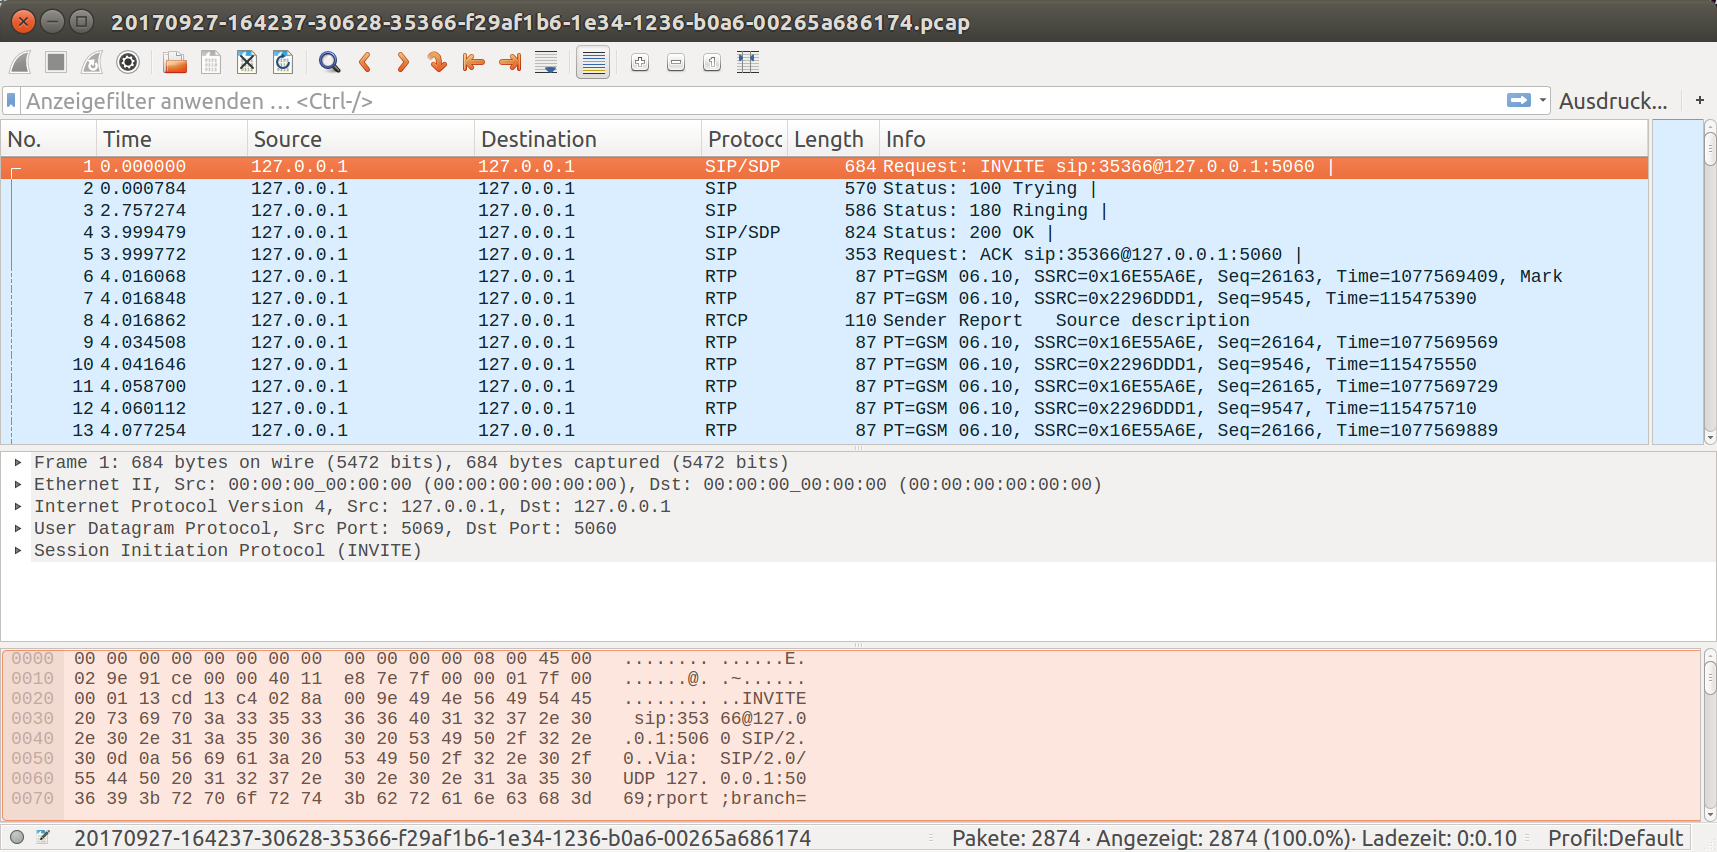
\includegraphics[width=15cm]{includes/w_SIPRTP}
\caption{Extrahierte SIP\- \& RTP\-Pakete}
\label{fig:wSipRTP}
\end{figure}

Die .raw-Dateien können nun via folgendem Komandozeilenaufruf abgespielt werden.
\begin{lstlisting}
padsp play -t gsm -r 8000 -c 1 example.gsm
\end{lstlisting}

Mit dem universellen Audiokonverter SoX können die Dateien in .wav convertiert werden, sodass diese auch mit jedem herkömmlichen Media Player abgespielt werden können.
\begin{lstlisting}
sox -t gsm -r 8000 -c 1 example.raw exampleConverted.wav
\end{lstlisting}

Mit dem Bash-Skript pcap2wav von Git \url{https://gist.github.com/avimar/d2e9d05e}\
\url{082ce273962d742eb9acac16} können genau diese Schritte automatisiert durchgeführt werden.


\subsection{Automatisierung}\label{automatisierung}

Das Abspeichern der Daten funktioniert bereits voll automatisiert und jeweils in eine extra Datei pro Session. Allerdings sollte das Konvertierungs-Skript noch automatisch ausgeführt werden. Hierfür kann das Linux-Tool \textit{Incron} genutzt werden. Das Tool setzt auf das Kernel-Subsystem Inotify, um auf Dateisystem-Ereignisse zu reagieren. Dadurch kann ein Ordner überwacht werden und beim Erstellen einer neuen Datei die Ausführung des Konvertierungs-Skriptes getriggert werden. Incron ähnelt dabei in der Handhabung an das Standardwerkzeug \textit{Cron}, welches Cron Jobs auf Basis von Zeitpunkten startet.


\begin{lstlisting}
sudo apt-get install -y incron
\end{lstlisting}

Damit das Programm gestartet und konfiguriert werden kann, muss in der Datei \textit{/etc/incron.allow} der Username eingetragen werden. Danach kann der Service gestartet werden.

\begin{lstlisting}
systemctl start incron.service
\end{lstlisting}

Analog zu \textit{Cron} werden über \textit{incrontab -e} die Jobs angelegt und verwaltet.
\begin{lstlisting}
/home/all/wiresharkCalls IN_CLOSE_WRITE /home/all/startPcap2wavgsmConversion.sh $@ $#
\end{lstlisting}


\begin{figure}[h] %t=top b=bottom h=here p =eigene page
\centering
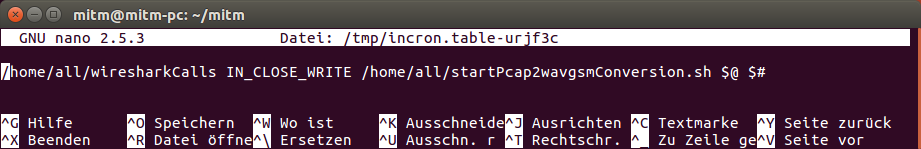
\includegraphics[width=15cm]{includes/incrontab}
\caption{Zeile des incrontab}
\label{fig:incrontab}
\end{figure}


Der Eintrag besteht aus dem zu beobachtenden Verzeichnis-Pfad, dem auftretendem Ereignis und zuletzt dem auszuführenden Befehl beziehungsweise Skript. Über den Parameter \textit{\$@}  wird das beobachtete Verzeichnis und mit \textit{\$\#} der Name der Datei, welches das Ereignis getriggert hat, übergeben. Das Konvertierungs-Skript von \ref{extractData} soll ausschließlich nach der Erstellung der Datei ausgeführt werden. Dazu wurde das Ereignis \textit{IN\_CLOSE\_WRITE} genutzt, das in Abbildung \ref{fig:incrontab} zu sehen ist. Sobald die Datei vollständig erstellt und geschlossen wurde, wird das auszuführende Skript (siehe Anhang \ref{startingConvertScript}) getriggert. Dieses übergibt dem Konvertierungs-Skript von \ref{extractData} die passenden Parameter und führt dieses aus.\\

Über den Status kann überprüft werden, ob ein Ereignis ausgelöst und das Skript getriggert wurde.

\begin{lstlisting}
systemctl status incron.service
\end{lstlisting}


Nun werden also die Daten direkt von der Schnittstelle abgegriffen, gefiltert und gespeichert. Danach automatisch in .wav konvertiert, sodass die Gespräche lokal auf dem PC angehört werden können. Damit wäre das Projektziel bereits erreicht beziehungsweise mit der Konvertierung auch praktisch erweitert. Um nicht an den lokalen PC gebunden zu sein, wäre es nun auch möglich die Dateien über einen Webserver global zur Verfügung zu stellen.


\subsection{Feature - Abhören der Aufnahme}
Es soll das letzte oder die letzten Gespräche via einem Telefonanruf wiedergegeben werden können. Dies wurde zuerst mit einer, anschließend für mehrere speziell konfigurierte Nummern ermöglicht. 
Durch Änderungen und Erweiterungen in der der Konfigurationsdatei "extensions.conf" von Asterisk konnte jeweils eine Rufnummer hinterlegt werden, unter der ein Gespräch bereitgestellt wird. Das Abspielen einer Datei erfolgt durch die Methode \textit{Playback}.\\

Da Asterisk kein .wav im GSM-Netz unterstützt, musste das Gepräch zusätzlich in .gsm konvertiert werden. Aus diesem Grund wurde das orignal Skript von \ref{extractData} angepasst, sodass mit diesem beide Konvertierungen möglich waren.\\

Die Realisierung hierfür unterscheidet sich jedoch stark von dem verwendeten Architekturansatz. Dies liegt an den unterschiedlichen Asterisk-Versionen, die verwendet wurden. Ein Tausch beider Konfigurationen schlug fehl. Nachfolgend sind beide Ansätze aufgelistet:




\textbf{Konfigurationsdatei für OsmoNITB-Ansatz}

\begin{lstlisting}
[gsmsubscriber]
exten=> 000001,1,Progress()
exten=> 000001,n,Wait(1)
exten=> 000001,n,Playback(/home/all/gsmCalls/recordedCall1.gsm_mixed)
exten=> 000001,n,Hangup()

exten=> 000002,1,Progress()
exten=> 000002,n,Wait(1)
exten=> 000002,n,Playback(/home/all/gsmCalls/recordedCall2.gsm_mixed)
exten=> 000002,n,Hangup()

exten=> 000003,1,Progress()
exten=> 000003,n,Wait(1)
exten=> 000003,n,Playback(/home/all/gsmCalls/recordedCall3.gsm_mixed)
exten=> 000003,n,Hangup()

exten=> 000004,1,Progress()
exten=> 000004,n,Wait(1)
exten=> 000004,n,Playback(/home/all/gsmCalls/recordedCall4.gsm_mixed)
exten=> 000004,n,Hangup()

exten=> 000005,1,Progress()
exten=> 000005,n,Wait(1)
exten=> 000005,n,Playback(/home/all/gsmCalls/recordedCall5.gsm_mixed)
exten=> 000005,n,Hangup()

exten=>_XXXXX,1,Dial(SIP/GSM/${EXTEN})
exten=>_XXXXX,n,HangUp
\end{lstlisting}

Insgesamt sind fünf Rufnummern (000001 - 000005) hinterlegt, sodass die letzten fünf Telefonate angehört werden können. Sie repräsentieren jeweils ein Mobiltelefon, das mit einer dieser Nummern verknüpft wurde. Diese Verknüpfung wird in der Datei "slots" hergestellt. Hier wird die IMSI einer Nummer zugeordnet. 
Nach Aufzeichnen eines Telefongesprächs und erneutem Anruf wird die erzeugte .gsm/wav Datei, des jeweiligen Slots überschrieben.



\textbf{Konfigurationsdatei für OpenBTS-Ansatz}

\begin{lstlisting}
[default](+)
exten => 000001,	1,Set(CDR(hangupdirection)=A)
same =>			n,Answer()
same =>			n,GotoIf($["${CDR(A-IMSI)}"!="IMSI010100000000006"]?BUSY)
same =>			n,Playback(/home/all/gsmCalls/recordedCall1.gsm_mixed)
same =>			n,Set(CDR(hangupdirection)=SYSTEM)
same =>			n,Hangup(16)

same =>			n(BUSY,Set(CDR(hangupdirection)=SYSTEM)
same =>			n,Busy(5)

exten => 000002,	1,Set(CDR(hangupdirection)=A)
same =>			n,Answer()
same =>			n,GotoIf($["${CDR(A-IMSI)}"!="IMSI010100000000006"]?BUSY)
same =>			n,Playback(/home/all/gsmCalls/recordedCall2.gsm_mixed)
same =>			n,Set(CDR(hangupdirection)=SYSTEM)
same =>			n,Hangup(16)

same =>			n(BUSY,Set(CDR(hangupdirection)=SYSTEM)
same =>			n,Busy(5)

exten => 000003,	1,Set(CDR(hangupdirection)=A)
same =>			n,Answer()
same =>			n,GotoIf($["${CDR(A-IMSI)}"!="IMSI010100000000006"]?BUSY)
same =>			n,Playback(/home/all/gsmCalls/recordedCall3.gsm_mixed)
same =>			n,Set(CDR(hangupdirection)=SYSTEM)
same =>			n,Hangup(16)

same =>			n(BUSY,Set(CDR(hangupdirection)=SYSTEM)
same =>			n,Busy(5)

exten => 000004,	1,Set(CDR(hangupdirection)=A)
same =>			n,Answer()
same =>			n,GotoIf($["${CDR(A-IMSI)}"!="IMSI010100000000006"]?BUSY)
same =>			n,Playback(/home/all/gsmCalls/recordedCall4.gsm_mixed)
same =>			n,Set(CDR(hangupdirection)=SYSTEM)
same =>			n,Hangup(16)

same =>			n(BUSY,Set(CDR(hangupdirection)=SYSTEM)
same =>			n,Busy(5)

exten => 000005,	1,Set(CDR(hangupdirection)=A)
same =>			n,Answer()
same =>			n,GotoIf($["${CDR(A-IMSI)}"!="IMSI010100000000006"]?BUSY)
same =>			n,Playback(/home/all/gsmCalls/recordedCall5.gsm_mixed)
same =>			n,Set(CDR(hangupdirection)=SYSTEM)
same =>			n,Hangup(16)

same =>			n(BUSY,Set(CDR(hangupdirection)=SYSTEM)
same =>			n,Busy(5)
\end{lstlisting}

In diesem Ansatz wurde die IMSI eines Mobilgeräts direkt hinterlegt, sodass nur dieser die Gespräche abhören kann. 






\subsection{Aufgetretene Probleme}

Ein Problem war, dass wir bei der Aufnahme der Daten zunächst nur UDP-Datenströme in Wireshark beobachten konnten. Die benötigten SIP-Daten waren nicht sichtbar. Dies konnten wir lösen, indem wir in Wireshark das Protokoll rtp\_udp aktivierten. Anschließend wurden die UDP-Daten als SIP-Daten dargestellt.

 -> Streams reichen nicht aus? (um alles automatisieren?!?) -> Installation von Sip-Connector\\



Konfigurationsprobleme -> Config Files bei einem System funktionieren auf dem eig. gleichen System auf einmal nicht mehr\\



Ein weiteres Problem ist, dass mit der OsmocomBB-Software es gelegentlich zu Verzögerungen beim Auflegen gab. Dies zeigte sich, indem es manchmal bis zu zehn Sekunden dauern konnte, ehe der Anruf aus der Mobiltelefonanzeige verschwand. Außerdem traten abhängig vom Mobiltelefon auch Störgeräusche auf.



Zuerst versucht zwischen BTS und BSC?!?
-> evtl Screenshot von Daten des ABIS-Interface?!
https://osmocom.org/projects/osmo-sip-conector/wiki/Osmo-sip-connector

http://ftp.osmocom.org/docs/latest/osmonitb-usermanual.pdf -> p.6/7 \\

Abgreifen der Daten zwischen BTS und BSC (ABIS-Interface) schwierig -> Daten weiter analysiert und weitere Angriffspunkte ausmachen.
-> Abgreifen der Daten vor der Telefonanlage (Asterisk (OPEN: IAX; Osmo: PBX)) -> dadurch die Daten im VOIP Format (SIP + RTP), welches via PC relativ gut zu handeln ist. \\

Zunächst eigenes analysieren der Daten. Suche nach pratkischem Tool im Internet
-> pcapsipdump\\




Mit dem Tool in \ref{extractData}, welches für das Abspeichern der Daten zuständig ist, gab es Probleme. Denn es wurde kein Datei-Ereignis beziehungsweise erst nach sehr langer Verzögerung erkannt. Nach Lesen und Debuggen des Source-Codes, stellte sich heraus, dass das Tool die erstellte Datei sehr lange nicht schließt, obwohl bereits seit längerem die Session beendet ist. Der Übeltäter war ein Timer in der calltable-Klasse, welcher auf 5 Minute gestellt war. Nach Verändern des Source-Codes und Anpassen des Timers auf 5 Sekunden wurde auch die erstellte pcap-Datei kurz nach Ende der Session geschlossen und das Incron-Ereignis zum Start der Konvertierung getriggert.

\begin{lstlisting}[xleftmargin=.04\textwidth, firstnumber=211]
  ...
 if (table[idx].is_used && (
 	(currtime - table[idx].last_packet_time > 5) ||
    (currtime - table[idx].first_packet_time > opt_absolute_timeout))){
  ...
\end{lstlisting}
